\section{Derivative Features: Justification and Construction}
\label{sec:derivative}


In this section we justify the inclusion of the time derivative $\dot{x}_{\mathrm{obs}}$ as an explicit input feature for the hidden-state estimator $H_\phi$.
We show that this architectural choice is not merely an empirical heuristic but is supported by an implicit-function argument.
We then describe the asymmetric construction of derivative features during training and inference to handle data sparsity, and we report
a toy ablation study on the SIR model.

\subsection{Justification via the implicit function theorem}
\label{subsec:derivative-justification}

Consider again the governing ODE for the full state $\mathbf{x}(t)=[x_{\mathrm{obs}}(t),x_{\mathrm{hid}}(t)]^\top$,
\[
\dot{\mathbf{x}}(t) = f(\mathbf{x}(t),\theta),
\]
and recall that $x_{\mathrm{obs}}(t)=h(\mathbf{x}(t))$ for the coordinate-projection observation operator $h$.
The observed dynamics can then be written as
\begin{equation}
\label{eq:obs-ode}
\dot{x}_{\mathrm{obs}}(t)
=
\frac{d}{dt}h(\mathbf{x}(t))
=
h\bigl(f(\mathbf{x}(t),\theta)\bigr)
=
h\bigl(f(x_{\mathrm{obs}}(t),x_{\mathrm{hid}}(t),\theta)\bigr).
\end{equation}

To express the hidden state $x_{\mathrm{hid}}$ in terms of observable quantities, we define the residual
\begin{equation}
\label{eq:residual}
F\bigl(x_{\mathrm{obs}},\dot{x}_{\mathrm{obs}},x_{\mathrm{hid}},\theta\bigr)
:=
\dot{x}_{\mathrm{obs}}
-
h\bigl(f(x_{\mathrm{obs}},x_{\mathrm{hid}},\theta)\bigr).
\end{equation}
We are interested in solving $F=0$ for $x_{\mathrm{hid}}$ as a function of $(x_{\mathrm{obs}},\dot{x}_{\mathrm{obs}},\theta)$.
By the implicit function theorem, if the Jacobian of $F$ with respect to $x_{\mathrm{hid}}$ is nonsingular at a point where $F=0$, i.e.,
\begin{equation}
\label{eq:jacobian-deriv}
\det\left(\frac{\partial F}{\partial x_{\mathrm{hid}}}\right)
=
\det\left(-\frac{\partial}{\partial x_{\mathrm{hid}}}\, h\bigl(f(x_{\mathrm{obs}},x_{\mathrm{hid}},\theta)\bigr)\right)
\neq 0,
\end{equation}
then there exists a locally unique, smooth function $g$ such that
\begin{equation}
\label{eq:IFT-repr}
x_{\mathrm{hid}} = g\bigl(x_{\mathrm{obs}},\dot{x}_{\mathrm{obs}},\theta\bigr)
\end{equation}
in a neighborhood of that point.

This representation dictates a natural input–output pairing for our hidden-state estimator.
By designing $H_\phi$ to take $(x_{\mathrm{obs}},\dot{x}_{\mathrm{obs}},\theta)$ as inputs and to approximate $x_{\mathrm{hid}}$,
we ensure that the network has the structural capacity to approximate the inverse mapping guaranteed by the implicit function theorem.

\subsection{Training-time construction: exact derivatives from the vector field}
\label{subsec:derivative-training}

During supervised training, the ground-truth parameter $\theta$ and full state $\mathbf{x}(t)$ are available for simulated trajectories.
In this setting, the observed derivative in \eqref{eq:obs-ode} can be evaluated directly from the vector field:
\[
\dot{x}_{\mathrm{obs}}(t_i)
=
h\bigl(f(\mathbf{x}(t_i),\theta)\bigr),
\]
which yields an exact (noise-free) derivative at each sampling time $t_i$.
We aggregate these values into the derivative feature matrix
\[
\dot{\mathbf{x}}_{\mathrm{obs}}
=
\bigl[\dot{x}_{\mathrm{obs}}(t_0),\ldots,\dot{x}_{\mathrm{obs}}(t_{N-1})\bigr]^\top,
\]
which is then used in the concatenated input $\mathbf{u}$ (Section~\ref{subsec:method-overview}).

This construction has two advantages in the training phase:
(i) it provides derivatives without numerical differentiation of sparse samples, and
(ii) it encourages $H_\phi$ to learn the inverse relation \eqref{eq:IFT-repr} under idealized conditions where the forward model is exact.

\subsection{Inference-time construction: spline-based approximation}
\label{subsec:derivative-inference}

At inference, neither $\theta$ nor $x_{\mathrm{hid}}(t)$ is known, so the vector-field formula for $\dot{x}_{\mathrm{obs}}(t)$ cannot be used directly.
Instead, we approximate derivatives from the sparse observations $\{x_{\mathrm{obs}}(t_i)\}_{i=0}^{N-1}$.

In our main experiments, we construct $\widehat{\dot{x}}_{\mathrm{obs}}(t_i)$ by first interpolating the observed trajectory with a cubic spline
and then differentiating the spline analytically.
This choice yields a smooth derivative estimate that respects the sampling grid and is robust to moderate noise.
We then form the feature matrix
\[
\widehat{\dot{\mathbf{x}}}_{\mathrm{obs}}
=
\bigl[\widehat{\dot{x}}_{\mathrm{obs}}(t_0),\ldots,\widehat{\dot{x}}_{\mathrm{obs}}(t_{N-1})\bigr]^\top,
\]
which is used in the concatenated input $\mathbf{u}$ at inference time.

Alternative constructions are possible, such as finite differences, polynomial or Lagrange interpolation, and higher-order smoothing schemes.
In Section \ref{subsec:derivative-ablation}, we evaluate the accuracy of these approximation schemes across multiple dynamical regimes, setting the stage for analyzing their ultimate impact on downstream hidden-state and parameter estimation.

\subsection{Evaluation of derivative approximations across dynamical regimes}
\label{subsec:derivative-ablation}

To illustrate the practical effect of derivative approximations, we evaluate the proposed cubic spline method against finite differences (FD) and Lagrange polynomial interpolation. Rather than limiting the analysis to a single system, we conduct a comprehensive evaluation across three distinct dynamical regimes: monotonic/bell-shaped (SIR), periodic (Lotka-Volterra), and delayed non-linear (OGTT). The goal is to determine which approximation scheme most reliably reconstructs the local vector field from sparse, noisy observations, a prerequisite for learning the inverse mapping in Equation~\eqref{eq:IFT-repr}.

\paragraph{Qualitative Analysis on Local Tangents} 
Figure~\ref{fig:all-tangent-ablation} visualizes the local directional derivatives (tangent lines) estimated at each sparse observation point. The implicit function formulation heavily relies on the instantaneous flow of the system. We observe that high-order Lagrange polynomials (magenta) exhibit severe Runge's phenomenon, generating wildly oscillating tangents particularly at the boundaries of the observation window. Finite differences (green) are directly susceptible to the injected observation noise, frequently deviating from the ground-truth vector field. In contrast, the cubic spline approximation (blue) smoothly interpolates the global trajectory, inherently filtering local noise and yielding tangent vectors that most closely align with the true physical flow (black).

\paragraph{Robust Quantitative Evaluation}
To rigorously quantify this observation, we perform a robust Monte Carlo evaluation. For each of the three dynamical systems, we sample $N=100$ independent trajectories with varying initial conditions and simulate realistic observation noise. Figure~\ref{fig:derivative_mse_dist} reports the distribution of the Mean Squared Error (MSE) between the estimated derivatives and the ground-truth vector field. 

The results reveal the distinct limitations of baseline methods. The Lagrange polynomial fails catastrophically across all systems, showing extreme variance and exponentially higher errors. While finite differences perform adequately in relatively simple, monotonic regimes (e.g., SIR, where it marginally matches spline performance), its error distribution significantly shifts upward in systems with high curvature or periodicity (Lotka-Volterra). 

Crucially, the cubic spline approach demonstrates \textit{universal robustness}. While it may not strictly reduce the error to zero, it consistently maintains the tightest error bounds and the lowest variance across all tested conditions—whether the underlying dynamics are monotonic, periodic, or governed by complex delays. This structural stability justifies our architectural choice: providing the hidden-state estimator $H_\phi$ with spline-based derivative features ensures a reliable and bounded input space, preventing the estimation network from diverging due to poorly approximated local flows.

% ---------------------------------------------------------
% Figure 1: 1x3 Qualitative Tangent Lines
% ---------------------------------------------------------
\begin{figure*}[htbp]
  \centering
  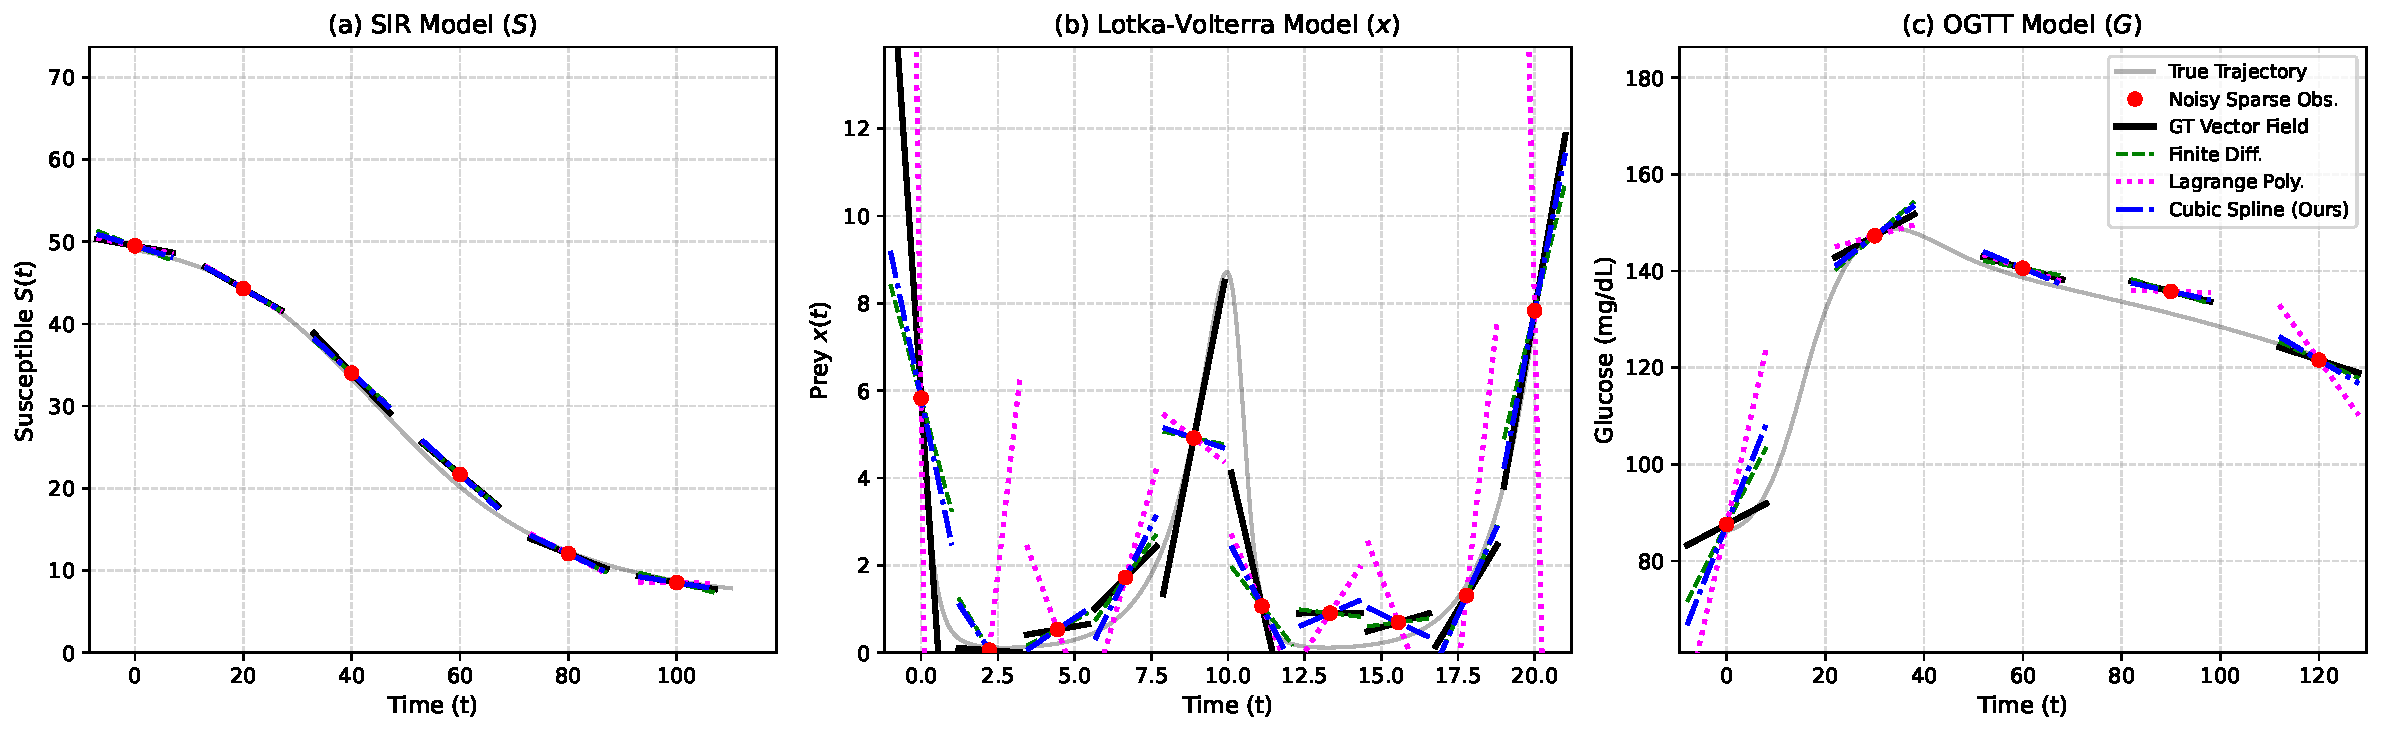
\includegraphics[width=\textwidth]{figures/all_systems_tangent_ablation.pdf}
  \caption{Qualitative comparison of local derivative approximations across three distinct dynamical systems: (a) SIR, (b) Lotka-Volterra, and (c) OGTT. 
  The black curves represent the ground-truth trajectories, and the red dots denote sparse, noisy observations encountered during inference.
  The tangent lines overlaid at each observation point visualize the local vector field estimated by different schemes. 
  Across all regimes—monotonic, periodic, and delayed non-linear—Lagrange polynomials (magenta) exhibit severe Runge's phenomenon at the boundaries, while finite differences (green) are highly susceptible to noise amplification. 
  Our cubic spline approach (blue) consistently yields the most robust approximation of the true vector field (black), providing stable structural priors for the implicit inverse mapping.}
  \label{fig:all-tangent-ablation}
\end{figure*}

% ---------------------------------------------------------
% Figure 2: Box plot for Quantitative MSE
% ---------------------------------------------------------
\begin{figure}[htbp]
  \centering
  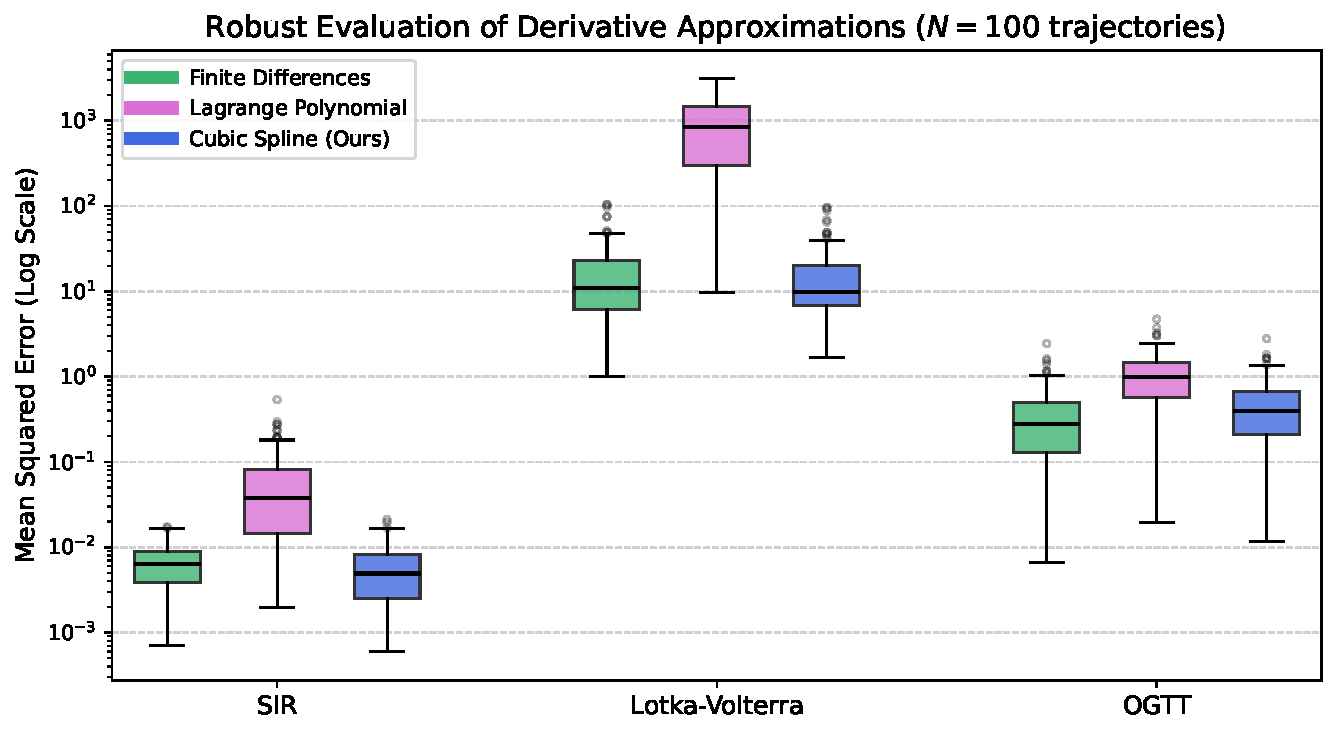
\includegraphics[width=0.85\textwidth]{figures/derivative_mse_distribution.pdf}
  \caption{Robust quantitative evaluation of derivative approximation accuracy. We compute the Mean Squared Error (MSE) between the estimated local derivatives and the ground-truth vector field across $N=100$ independent trajectories for each dynamical system. The box plots, scaled logarithmically on the y-axis, show the distribution of errors. Lagrange polynomial approximation suffers from catastrophic instability, exhibiting extreme variance. Finite differences adequately capture simple monotonic trends but struggle with periodicity and high curvature. In contrast, the cubic spline approach provides the most stable and consistent estimation of the implicit vector field across all regimes, maintaining tight error bounds even under severe data sparsity.}
  \label{fig:derivative_mse_dist}
\end{figure}

Having established the universal robustness of the cubic spline approximation for recovering the local vector field, we empirically demonstrate its direct impact on the network's downstream estimation performance in the following section.

\subsection{Impact of derivative features on downstream estimation}
\label{subsec:downstream-performance}

Having established the accuracy and robustness of the cubic spline approximation for local vector fields, we now evaluate its ultimate impact on the network's downstream tasks: hidden-state reconstruction and parameter estimation.

\paragraph{Experimental Setup}
To isolate the effect of derivative features during inference, we compare the performance of the hidden-state estimator $H_\phi$ under different input configurations on the OGTT benchmark. 
The baseline network (\textbf{No Deriv}) is trained and evaluated using only the observable state $x_{\mathrm{obs}}$. 
The derivative-augmented networks are evaluated by substituting the exact derivatives used in training with various approximation schemes, e.g., finite difference (\textbf{FD}), derivative of Lagrange interpolation (\textbf{LI}), and derivative of cubic spline (\textbf{CS}) computed from sparse, noisy test data.
Performance is measured using the Pearson correlation coefficient $R$ between ground-truth and estimated values for system parameters: insulin sensitivity $S_I$ and the beta-cell function $\sigma$.

\paragraph{Results and Discussion}
Table \ref{tab:ogtt_performance} summarizes the results across two test beds: noise-free simulation data and the NIH real-world clinical dataset.

\begin{table}[H]
\centering
\caption{Parameter estimation performance (Pearson $R$) on the OGTT benchmark. 
We compare the hidden-state estimator without derivative features (\textit{No Deriv}) against those using various derivative approximation schemes (Lagrange, Finite Difference, and Cubic Spline).}
\label{tab:ogtt_performance}
\begin{tabular}{@{}lcccc@{}}
\toprule
& \multicolumn{2}{c}{\textbf{Simulation Data}} & \multicolumn{2}{c}{\textbf{Real Data (NIH)}} \\ \cmidrule(lr){2-3} \cmidrule(lr){4-5} 
\textbf{Method} & $S_I$ & $\sigma$ & $S_I$ & $\sigma$ \\ \midrule
No Deriv & 0.697 & \textbf{0.544} & \textbf{0.583} & \textbf{0.505} \\
Lagrange Poly. & \textbf{0.700} & 0.538 & 0.577 & 0.490 \\
Finite Difference & \textbf{0.700} & 0.538 & 0.577 & 0.491 \\
Cubic Spline (Ours) & \textbf{0.700} & 0.538 & 0.576 & 0.490 \\ \bottomrule
\end{tabular}
\end{table}

\textbf{NEED DISCUSSION}